%3. Although I appreciate the robustness check to the various difference-in-differences estimators presented in Appendix B, it would be more reassuring to see the event studies.

Thank you very much for the suggestion. In the revised manuscript, we have expanded the ``Alternative Estimation Methods'' subsection of Appendix \ref{sec:appendixC} to include event-study plots for all main outcomes under each alternative estimator. We have also added a sentence in the Empirical Strategy section noting that the event studies using these staggered difference-in-differences estimators confirm flat pre-adoption trends under all estimation methods.

We reproduce this sentence from the Empirical Strategy section below:

\begin{adjustwidth}{2em}{0em}
Online Appendix Figure \ref{fig:figureA2_alterestim} shows robustness to alternative estimators, including those developed by \citet{Chaisemartin, Gardner, wooldridge2023simple}, as well as to the canonical two-way fixed effects (TWFE) estimator. The resulting estimates are remarkably similar across the alternative staggered-adoption estimators, except for the canonical TWFE, which shows attenuated effects, arguably driven by the negative weights problem discussed above \citep{GoodmanBacon}. The corresponding event studies, reported in Online Appendix Figures \ref{fig:alterestim_delitos}, \ref{fig:alterestim_inseguridad}, \ref{fig:alterestim_medidas}, and \ref{fig:alterestim_crime}, confirm that pre-adoption trends are flat under each alternative estimator.
\end{adjustwidth}

We also reproduce below the expanded ``Alternative Estimation Methods'' subsection of Online Appendix C:

\begin{adjustwidth}{2em}{0em}
The results reported in Section \ref{main_results} are estimated using the difference-in-differences estimator for staggered treatment adoption developed in \citet{Callaway}. In this subsection, we examine the robustness of the results to the use of alternative difference-in-difference estimators for staggered treatment adoption including those developed in \citet{Chaisemartin}, \citet{Gardner}, \citet{wooldridge2023simple}, and also to the canonical two-way fixed effects (TWFE).

The results of these analyses are reported in Figure \ref{fig:figureA2_alterestim} and show similar effects of \emph{Plan Cuadrante} in terms of both magnitude and statistical significance across most specifications. On the other hand, the canonical TWFE shows smaller effects, likely due to the negative weights problem highlighted by \citet{GoodmanBacon} when estimating difference-in-differences with staggered treatment adoption using TWFE.

Figures \ref{fig:alterestim_delitos} through \ref{fig:alterestim_crime} report the corresponding event-study estimates for victimization, crime perception, investment in security measures, and reported crime under each alternative estimator. Pre-treatment coefficients are consistently small and statistically indistinguishable from zero across all estimators and outcomes, confirming that the parallel trends assumption holds regardless of the estimation method. Post-treatment effects remain negative and statistically significant across these outcomes, closely mirroring the results from the main specification in Figure \ref{fig:figure02}.
\end{adjustwidth}

\clearpage
\noindent\textbf{Other figures referenced above:}
\vspace{0.5em}

{\renewcommand{\thefigure}{C.2}
\begin{figure}[h!]
    \centering
    \caption[Effects of \emph{Plan Cuadrante} on Police Effectiveness Using Alternative Estimators]{Effects of \emph{Plan Cuadrante} on Police Effectiveness Using Alternative Estimators}
    \label{fig:figureA2_alterestim}
    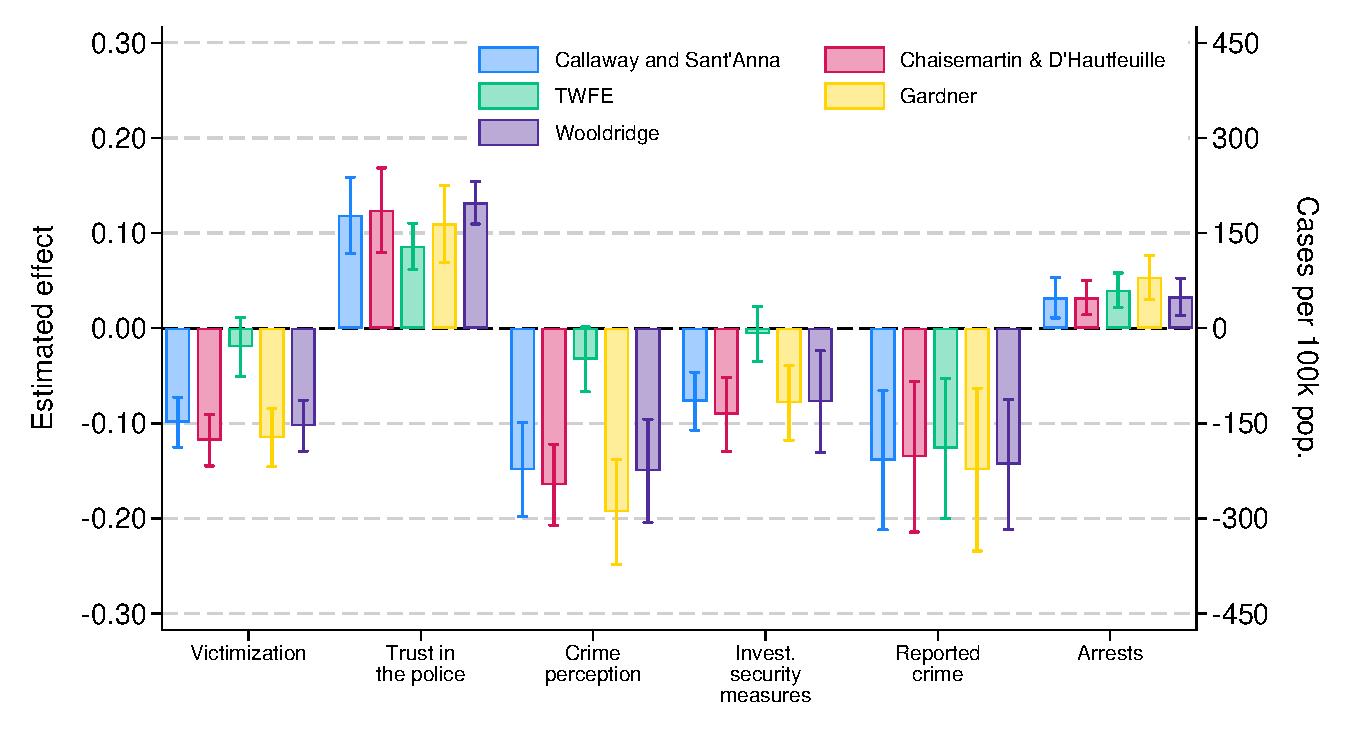
\includegraphics[width=\textwidth]{../manuscript/Graphs/Comparison_estimators_combined.pdf}
    \\[8pt]
    \begin{minipage}{0.99\textwidth}
    \footnotesize Notes: The figure reports the effects of \emph{Plan Cuadrante} on different measures of police effectiveness using various difference-in-differences estimators, including the methods developed in \citet{Callaway}, \citet{Chaisemartin}, \citet{Gardner}, \citet{wooldridge2023simple}, and the canonical two-way fixed effects (TWFE). Bars are the estimated post-treatment effects and the whiskers the 95\% confidence intervals; standard errors are clustered at the municipality level. Victimization is the probability of household victimization in the last 12 months; reported crime is the number of crimes reported to the police in the municipality per 100,000 inhabitants; crime perception is the probability of perceiving an increase in crime; investment in security measures is the probability of adopting security measures in the last twelve months; trust in the police is the probability of reporting high trust in the police; and arrests is the number of arrests per 100,000 inhabitants. Reported crime and arrests (administrative data) are read on the right axis; all other outcomes, from the ENUSC survey, are read on the left axis.
    \end{minipage}
\end{figure}
}

\clearpage

{\setcounter{figure}{2}\renewcommand{\thefigure}{C.\arabic{figure}}
% =============================================================================
% Alternative-estimator robustness figures
% Each figure shows the event study from three estimators:
%   (a) Chaisemartin & D'Hautfeuille
%   (b) Gardner
%   (c) Wooldridge
% Callaway & Sant'Anna is excluded — it appears as the headline figure.
%
% First block (3 figures): ENUSC survey outcomes
% Second block (1 figure): SPD administrative crime outcomes
% =============================================================================


% ----- Victimization (delitos) -----------------------------------------------
\begin{figure}[h!]
    \centering
    \caption[Effects of \emph{Plan Cuadrante} on Victimization Using Alternative Estimators]{Effects of \emph{Plan Cuadrante} on Victimization Using Alternative Estimators}
    \label{fig:alterestim_delitos}
    \begin{subfigure}{0.47\textwidth}
        \centering
        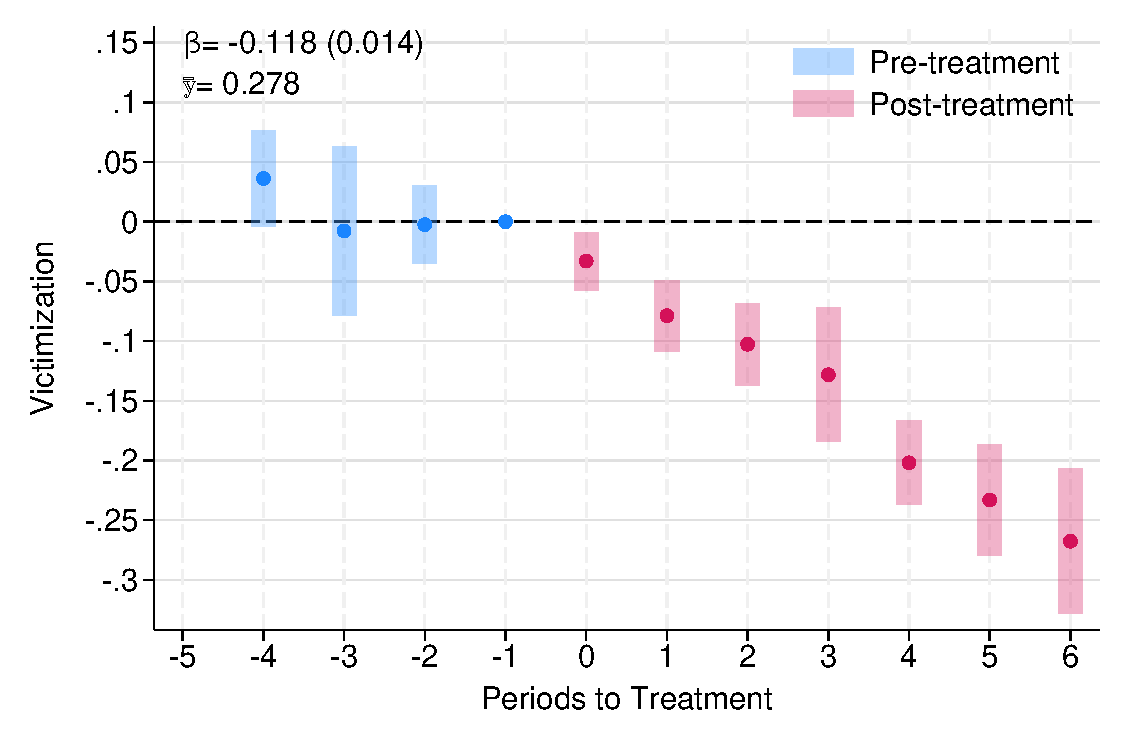
\includegraphics[width=\textwidth]{../manuscript/Graphs/CHDH_event_study_delitos.pdf}
        \caption{Chaisemartin \& D'Hautfeuille}
    \end{subfigure}%
    \begin{subfigure}{0.47\textwidth}
        \centering
        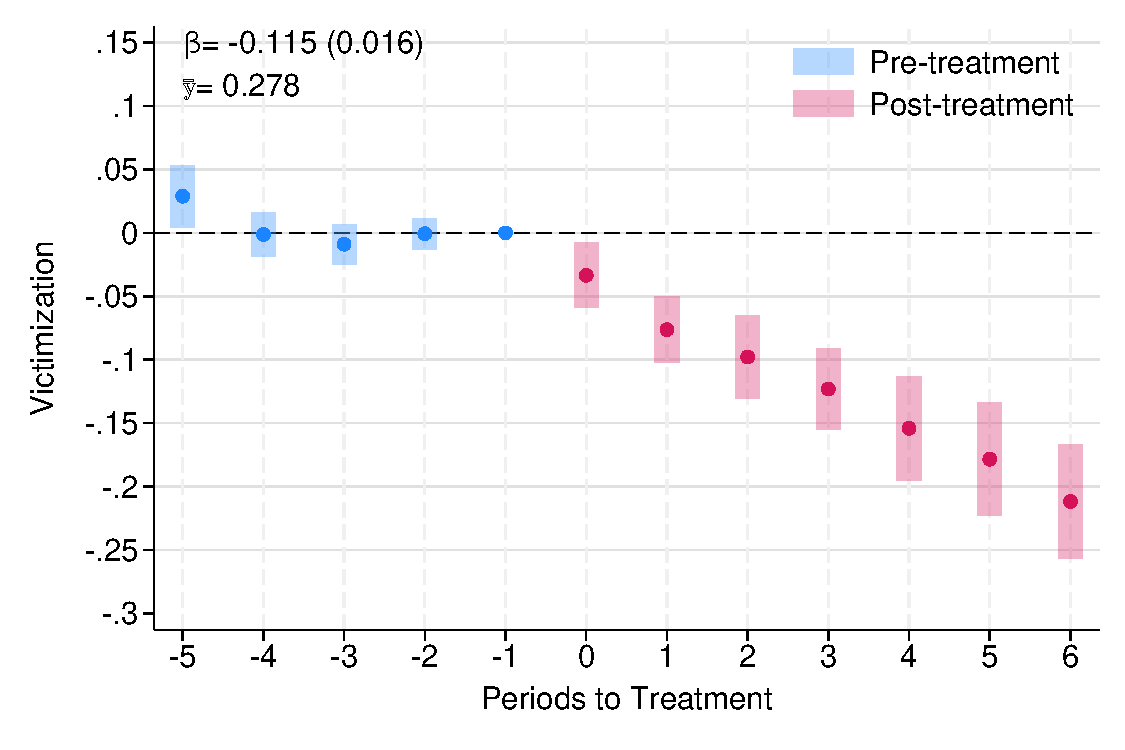
\includegraphics[width=\textwidth]{../manuscript/Graphs/DID2S_event_study_delitos.pdf}
        \caption{Gardner}
    \end{subfigure}
    \\[6pt]
    \begin{subfigure}{0.47\textwidth}
        \centering
        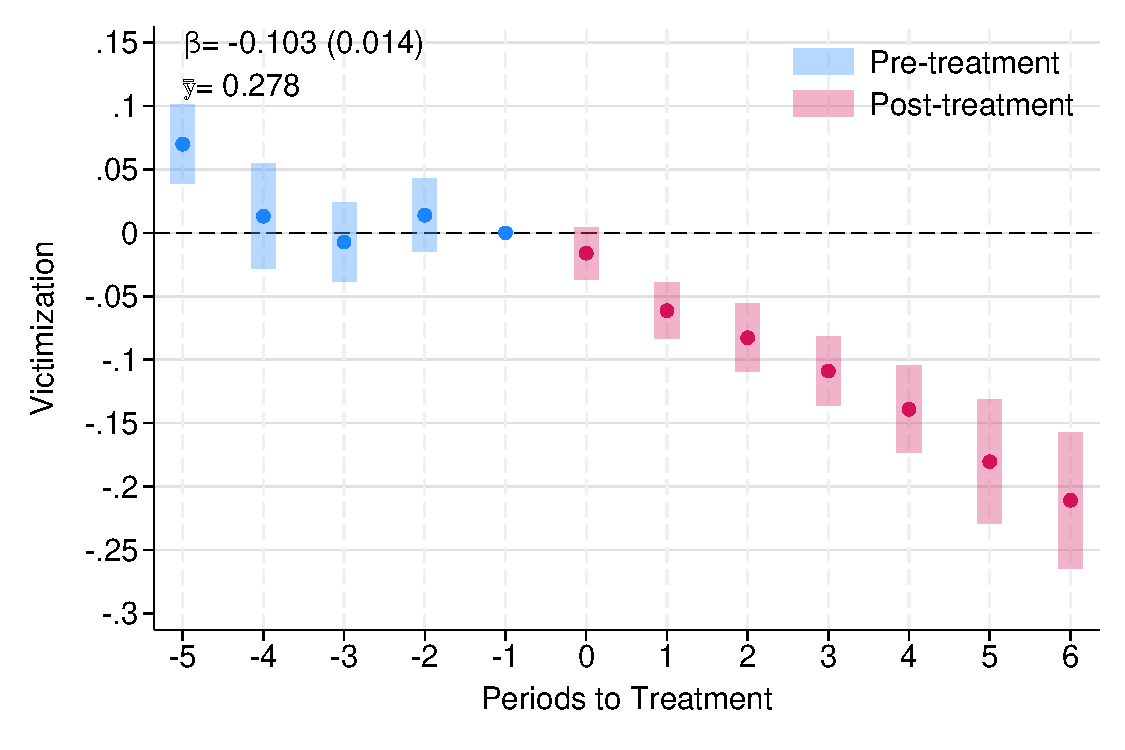
\includegraphics[width=\textwidth]{../manuscript/Graphs/JWDID_event_study_delitos.pdf}
        \caption{Wooldridge}
    \end{subfigure}
    \\[12pt]
    \begin{minipage}{0.99\textwidth}
    \footnotesize Notes: The figure reports event-study estimates of the effect of \emph{Plan Cuadrante} on the probability of household victimization in the last 12 months using the ENUSC survey, estimated with three alternative difference-in-differences estimators robust to staggered adoption: \citet{Chaisemartin} in panel (a), \citet{Gardner} in panel (b), and \citet{wooldridge2023simple} in panel (c). Each panel plots the estimated coefficient at each event time relative to treatment along with 95\% confidence intervals. Standard errors are clustered at the municipality level. The headline coefficient $\beta$ corresponds to the average post-treatment effect, and $\bar{y}$ denotes the never-treated mean of the outcome over the sample period.
    \end{minipage}
\end{figure}


% ----- Crime perception (inseguridad_barrio1) --------------------------------
\begin{figure}[h!]
    \centering
    \caption[Effects of \emph{Plan Cuadrante} on Crime Perception Using Alternative Estimators]{Effects of \emph{Plan Cuadrante} on Crime Perception Using Alternative Estimators}
    \label{fig:alterestim_inseguridad}
    \begin{subfigure}{0.47\textwidth}
        \centering
        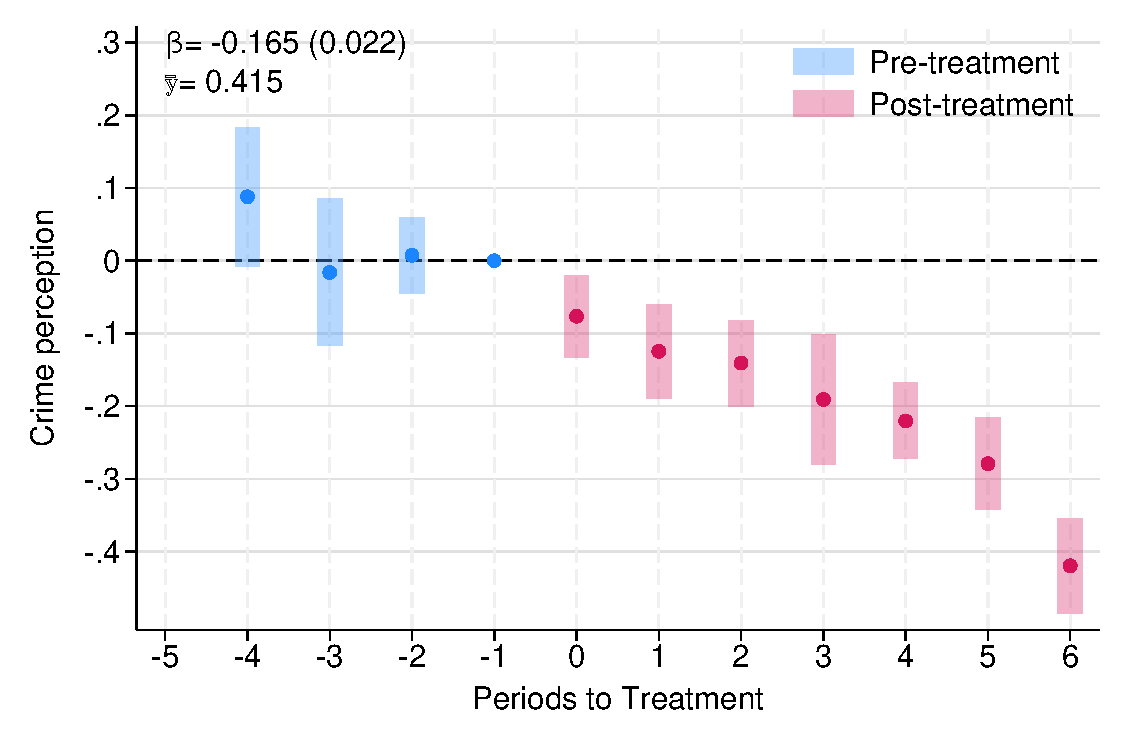
\includegraphics[width=\textwidth]{../manuscript/Graphs/CHDH_event_study_inseguridad_barrio1.pdf}
        \caption{Chaisemartin \& D'Hautfeuille}
    \end{subfigure}%
    \begin{subfigure}{0.47\textwidth}
        \centering
        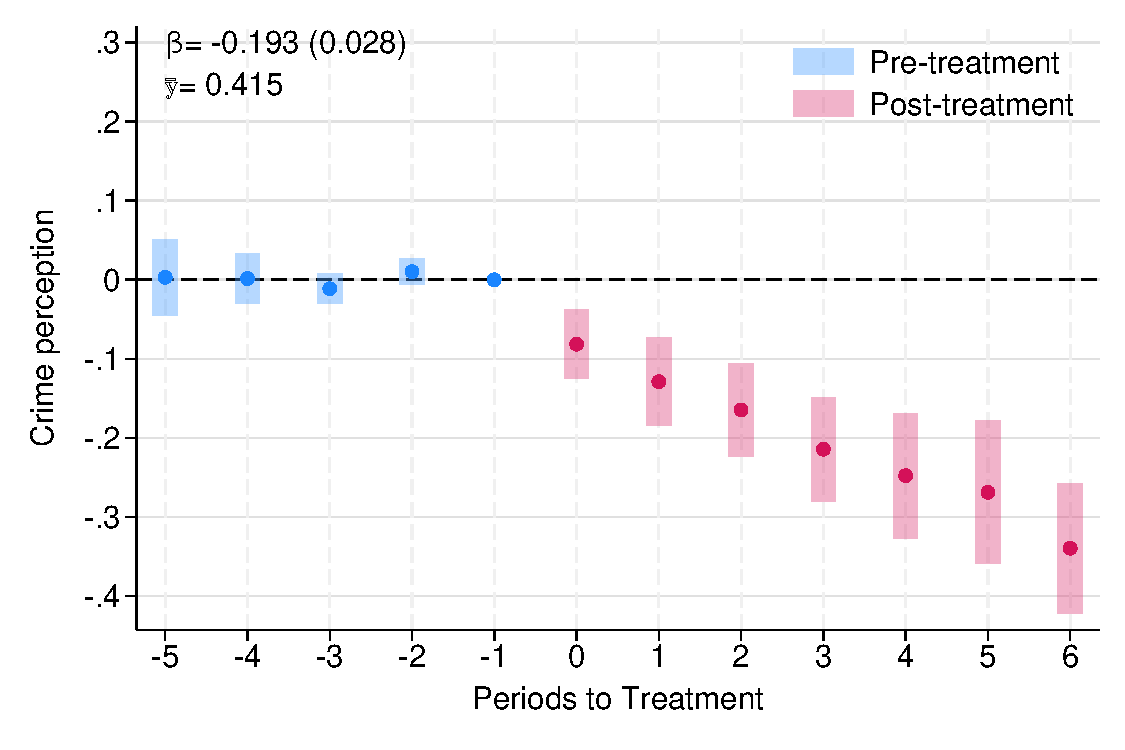
\includegraphics[width=\textwidth]{../manuscript/Graphs/DID2S_event_study_inseguridad_barrio1.pdf}
        \caption{Gardner}
    \end{subfigure}
    \\[6pt]
    \begin{subfigure}{0.47\textwidth}
        \centering
        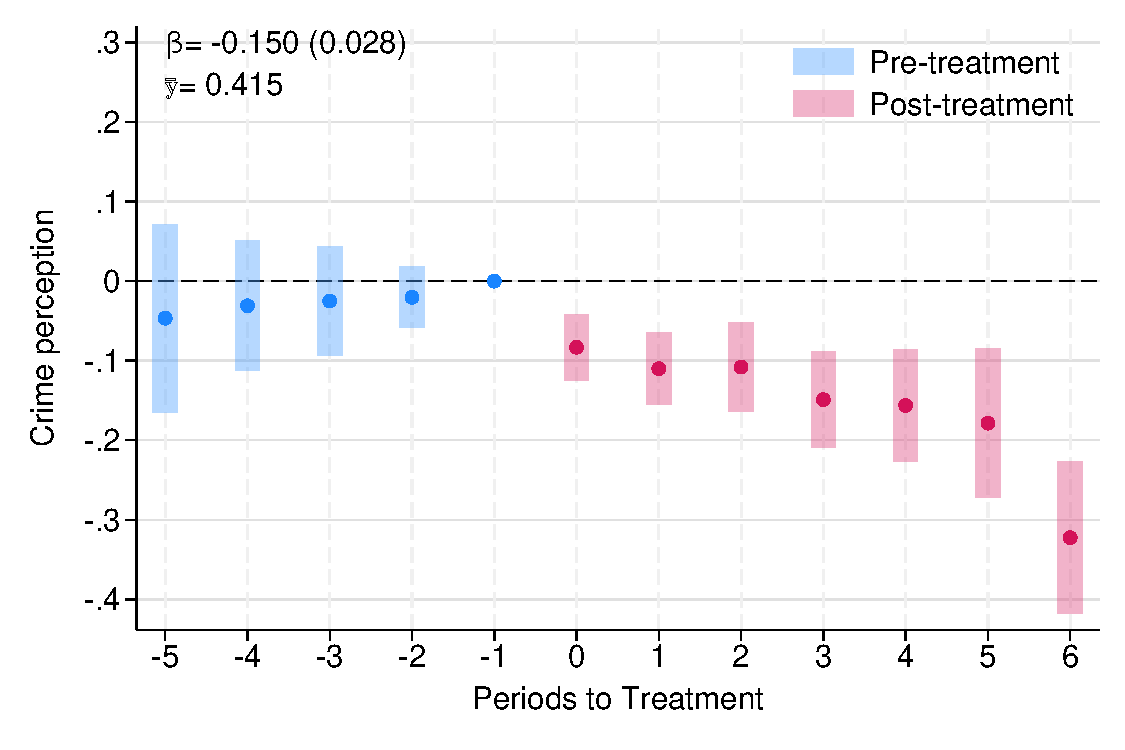
\includegraphics[width=\textwidth]{../manuscript/Graphs/JWDID_event_study_inseguridad_barrio1.pdf}
        \caption{Wooldridge}
    \end{subfigure}
    \\[12pt]
    \begin{minipage}{0.99\textwidth}
    \footnotesize Notes: The figure reports event-study estimates of the effect of \emph{Plan Cuadrante} on the probability of perceiving an increase in crime using the ENUSC survey, estimated with three alternative difference-in-differences estimators robust to staggered adoption: \citet{Chaisemartin} in panel (a), \citet{Gardner} in panel (b), and \citet{wooldridge2023simple} in panel (c). Each panel plots the estimated coefficient at each event time relative to treatment along with 95\% confidence intervals. Standard errors are clustered at the municipality level. The headline coefficient $\beta$ corresponds to the average post-treatment effect, and $\bar{y}$ denotes the never-treated mean of the outcome over the sample period.
    \end{minipage}
\end{figure}


% ----- Private investment in security (medidas_general_12) -------------------
\begin{figure}[h!]
    \centering
    \caption[Effects of \emph{Plan Cuadrante} on Investment in Security Measures Using Alternative Estimators]{Effects of \emph{Plan Cuadrante} on Investment in Security Measures Using Alternative Estimators}
    \label{fig:alterestim_medidas}
    \begin{subfigure}{0.47\textwidth}
        \centering
        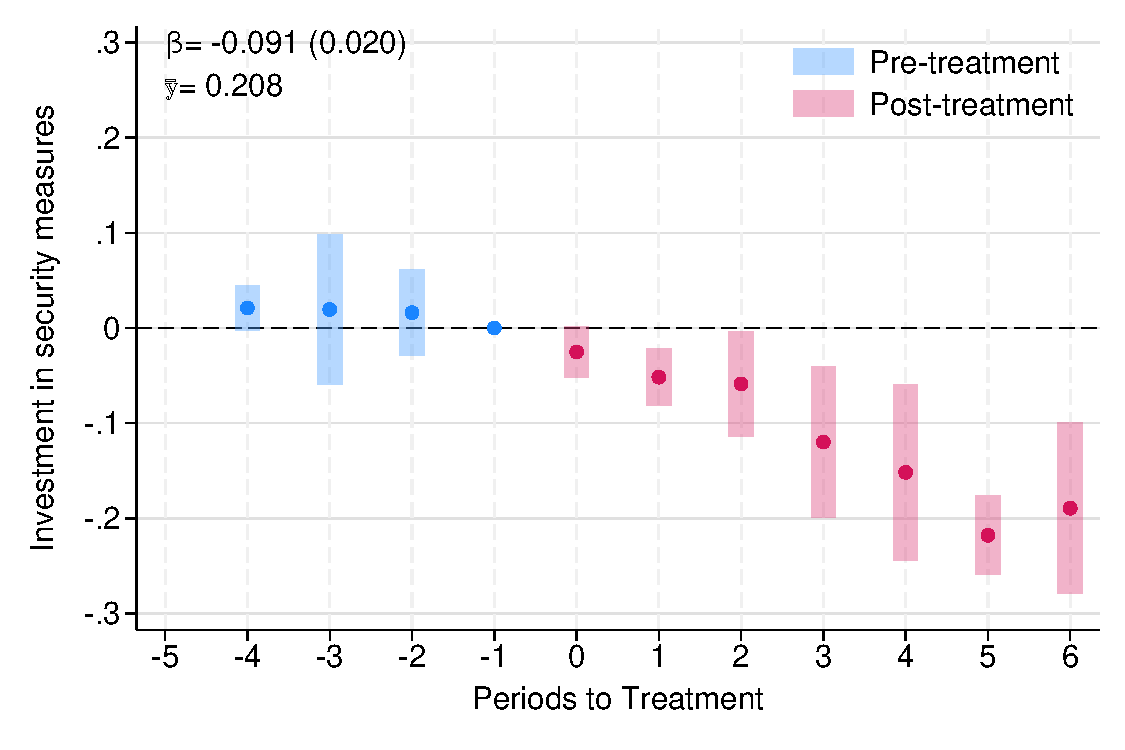
\includegraphics[width=\textwidth]{../manuscript/Graphs/CHDH_event_study_medidas_general_12.pdf}
        \caption{Chaisemartin \& D'Hautfeuille}
    \end{subfigure}%
    \begin{subfigure}{0.47\textwidth}
        \centering
        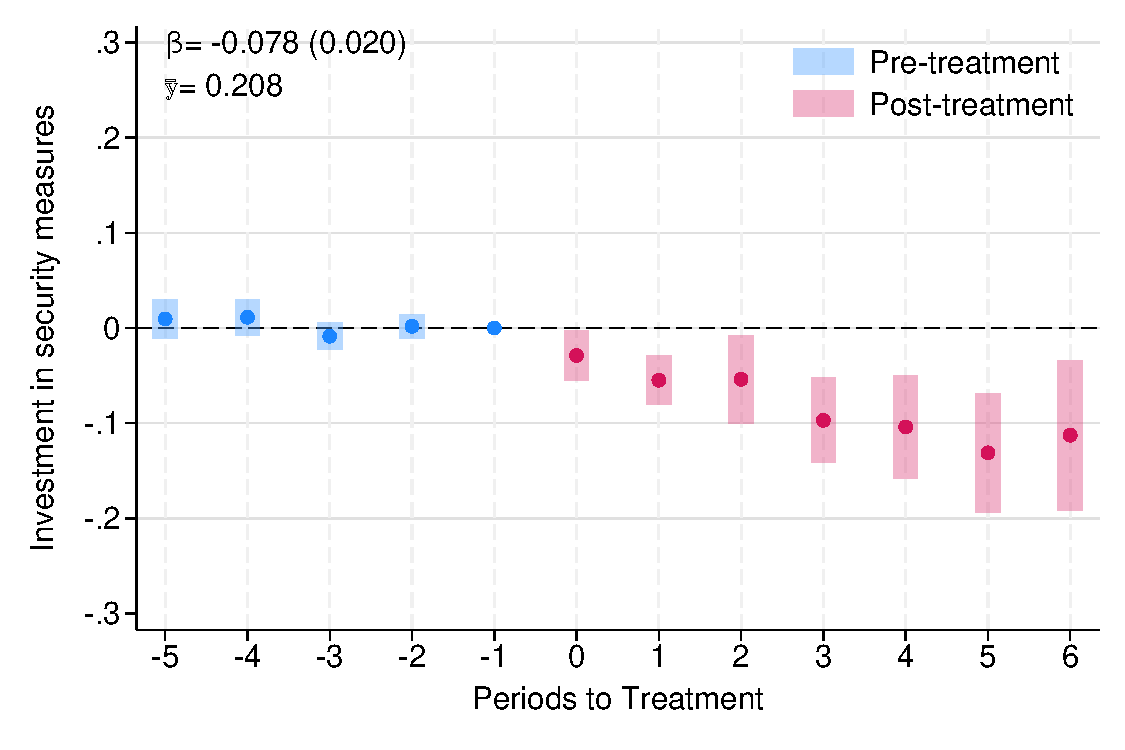
\includegraphics[width=\textwidth]{../manuscript/Graphs/DID2S_event_study_medidas_general_12.pdf}
        \caption{Gardner}
    \end{subfigure}
    \\[6pt]
    \begin{subfigure}{0.47\textwidth}
        \centering
        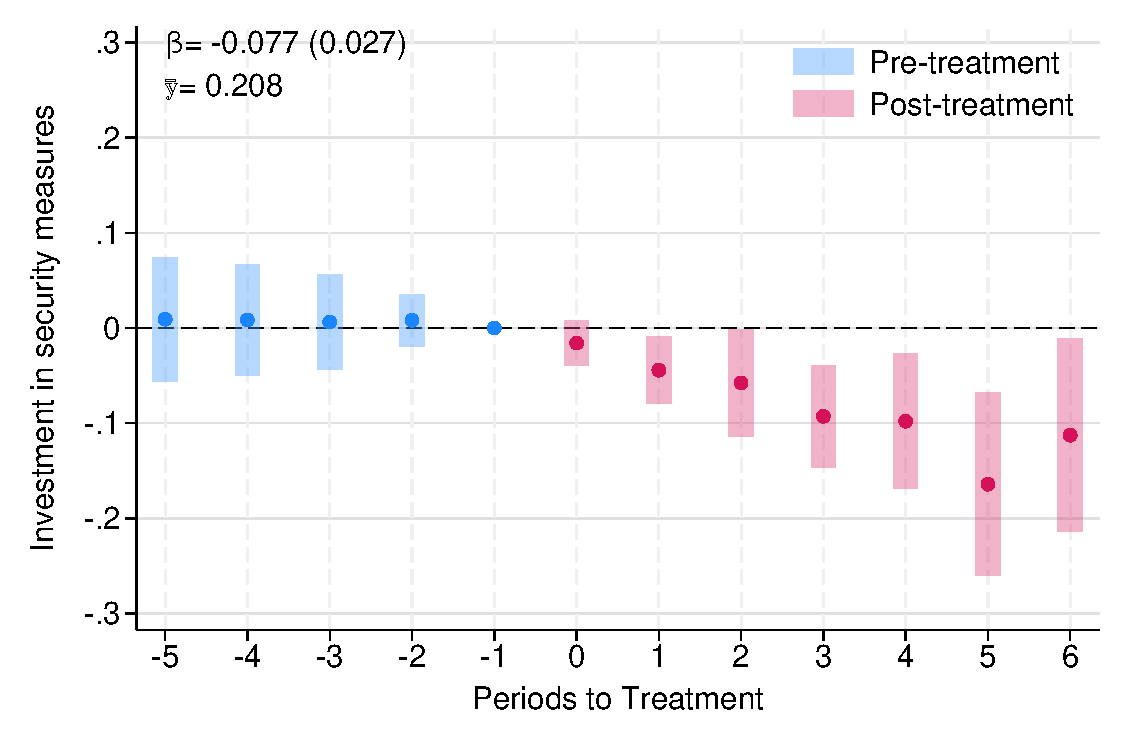
\includegraphics[width=\textwidth]{../manuscript/Graphs/JWDID_event_study_medidas_general_12.pdf}
        \caption{Wooldridge}
    \end{subfigure}
    \\[12pt]
    \begin{minipage}{0.99\textwidth}
    \footnotesize Notes: The figure reports event-study estimates of the effect of \emph{Plan Cuadrante} on the probability of adopting security measures in the last twelve months using the ENUSC survey, estimated with three alternative difference-in-differences estimators robust to staggered adoption: \citet{Chaisemartin} in panel (a), \citet{Gardner} in panel (b), and \citet{wooldridge2023simple} in panel (c). Each panel plots the estimated coefficient at each event time relative to treatment along with 95\% confidence intervals. Standard errors are clustered at the municipality level. The headline coefficient $\beta$ corresponds to the average post-treatment effect, and $\bar{y}$ denotes the never-treated mean of the outcome over the sample period.
    \end{minipage}
\end{figure}


% =============================================================================
% Administrative data (SPD municipality-level)
% =============================================================================


% ----- Reported crime --------------------------------------------------------
\begin{figure}[h!]
    \centering
    \caption[Effects of \emph{Plan Cuadrante} on Reported Crime Using Alternative Estimators]{Effects of \emph{Plan Cuadrante} on Reported Crime Using Alternative Estimators}
    \label{fig:alterestim_crime}
    \begin{subfigure}{0.47\textwidth}
        \centering
        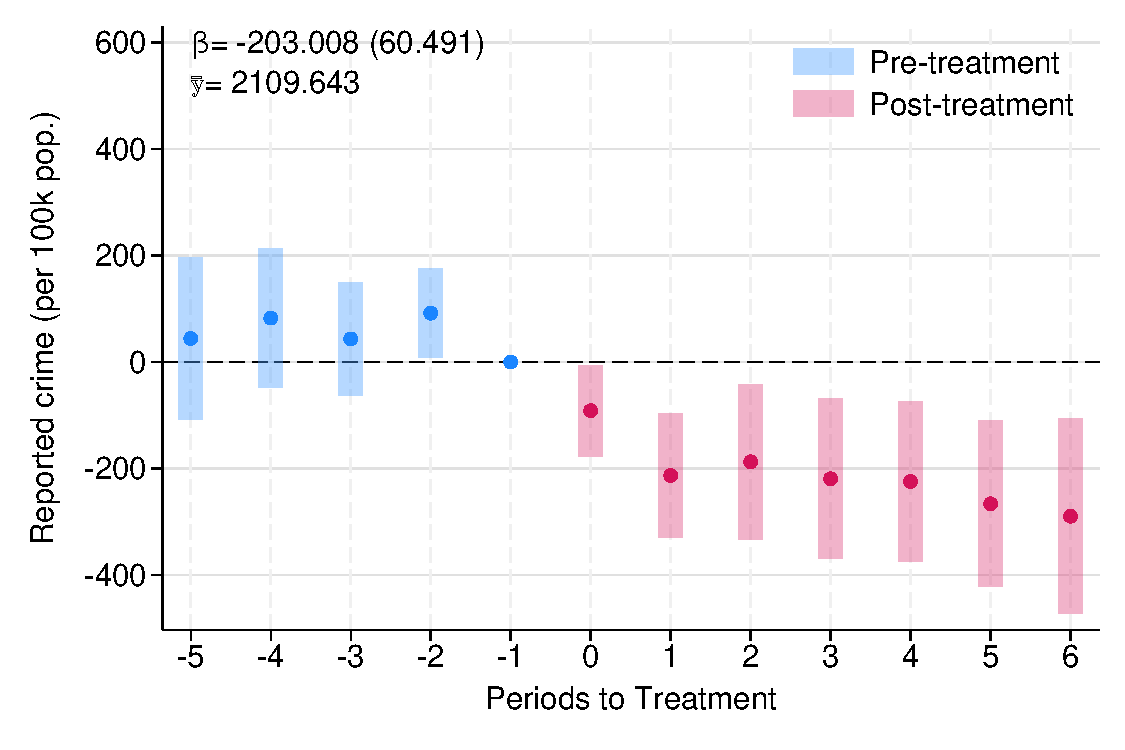
\includegraphics[width=\textwidth]{../manuscript/Graphs/CHDH_event_study_crime.pdf}
        \caption{Chaisemartin \& D'Hautfeuille}
    \end{subfigure}%
    \begin{subfigure}{0.47\textwidth}
        \centering
        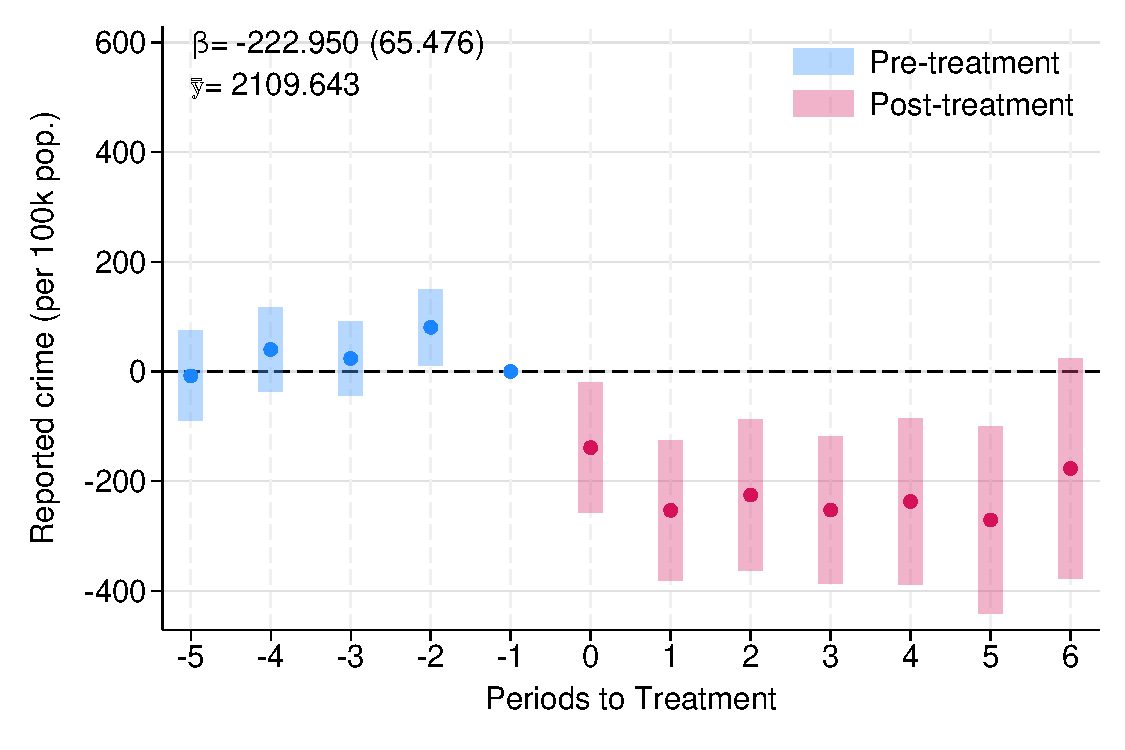
\includegraphics[width=\textwidth]{../manuscript/Graphs/DID2S_event_study_crime.pdf}
        \caption{Gardner}
    \end{subfigure}
    \\[6pt]
    \begin{subfigure}{0.47\textwidth}
        \centering
        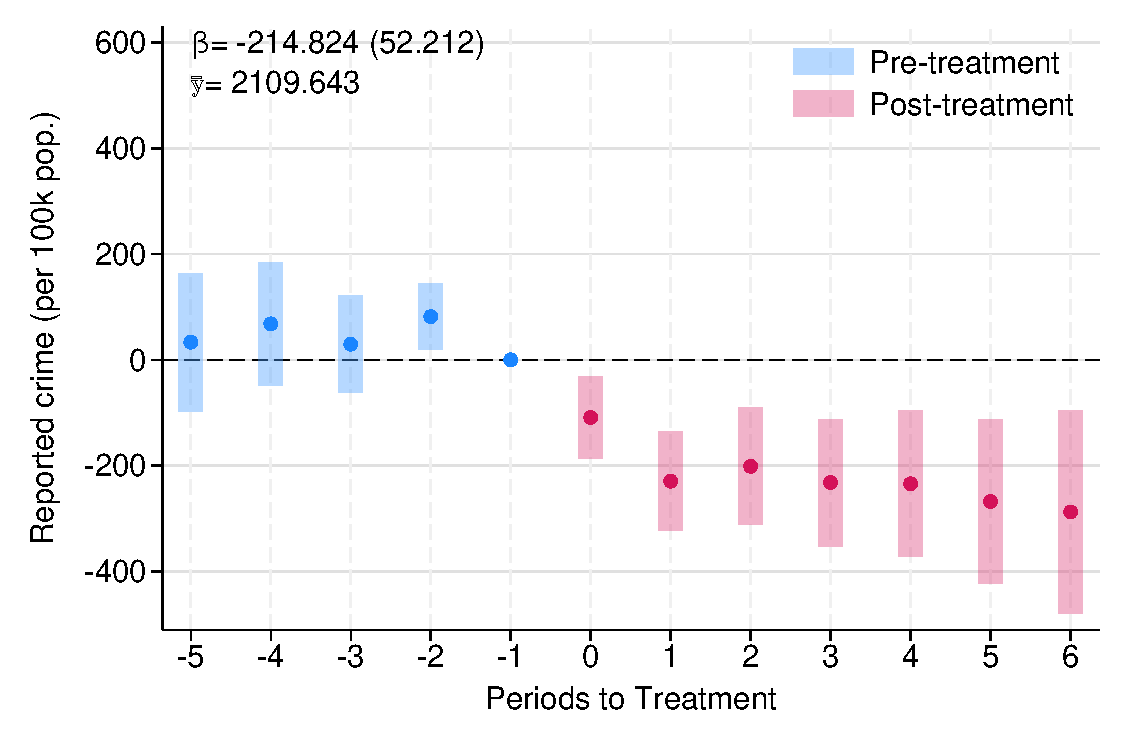
\includegraphics[width=\textwidth]{../manuscript/Graphs/JWDID_event_study_crime.pdf}
        \caption{Wooldridge}
    \end{subfigure}
    \\[12pt]
    \begin{minipage}{0.99\textwidth}
    \footnotesize Notes: The figure reports event-study estimates of the effect of \emph{Plan Cuadrante} on the number of crimes reported to the police in the municipality per 100,000 inhabitants using administrative data, estimated with three alternative difference-in-differences estimators robust to staggered adoption: \citet{Chaisemartin} in panel (a), \citet{Gardner} in panel (b), and \citet{wooldridge2023simple} in panel (c). Each panel plots the estimated coefficient at each event time relative to treatment along with 95\% confidence intervals. Standard errors are clustered at the municipality level. The headline coefficient $\beta$ is the equal-weighted average of the post-treatment effects from $t=0$ to $t=6$, and $\bar{y}$ denotes the never-treated mean of the outcome over the sample period.
    \end{minipage}
\end{figure}
}

\clearpage
